\documentclass[11pt]{article}
\usepackage{header}
\def\title{HW 13}

\begin{document}
\maketitle
\fontsize{12}{15}\selectfont

\begin{center}
    Due: Saturday, 4/26, 4:00 PM \\
    Grace period until Saturday, 4/26, 6:00 PM \\
\end{center}

\section*{Sundry}
Before you start writing your final homework submission, state briefly how you 
worked on it. Who else did you work with?  List names and email addresses. (In 
case of homework party, you can just describe the group.)

\begin{center}
    \textcolor{blue}{
        Zachary Brandt \\
        \nolinkurl{zbrandt@berkeley.edu}
    }
\end{center}

\vspace{15pt}

\Question{Estimating \texorpdfstring{$\pi$}{pi}}

\notelinks{\href{https://www.eecs70.org/assets/pdf/notes/n17.pdf}{Note 17}}
In this problem, we discuss one way that you could probabilistically estimate 
$\pi$. We'll use a square dartboard of side length 2, and a circular target 
drawn inscribed in the square dartboard with radius 1. A dart is then thrown 
uniformly at random in the square. Let $p$ be the probability that the dart 
lands inside the circle.

\begin{Parts}
    \item What is $p$?
	\item Suppose we throw $N$ darts uniformly at random in the square. Let 
    $\hat{p}$ be the proportion of darts that land inside the circle. Create an 
    unbiased estimator $X$ for $\pi$ using $\hat{p}$.
	\item Using Chebyshev's Inequality, compute the minimum value of $N$ such 
    that your estimate is within $\varepsilon$ of $\pi$ with $1 - \delta$ 
    confidence. Your answer should be in terms of $\varepsilon$ and $\delta$. 
    Note that since we are estimating $\pi$, your answer should not have $\pi$ 
    in it.
\end{Parts}

\begin{solution}

\begin{Parts}
    
\Part The probability that the dart lands in the circle is $p=
\frac{\pi \cdot 1^2}{2^2} = \frac{\pi}{4}$.

\Part An unbiased estimator $X$ for $\pi$ using $\hat{p}$ would be $X = 4\hat{p}$. 
The expected value of $X$ is $\E[X] =  4 \E[\hat{p}] =  4 p = \pi$ since, 
$\hat{p} = \frac{1}{N} \sum_{i=0}^{N} X_i$, where $X_i$ is an indicator variable
for if the $i$th dart is in the circle or not, with probability $p$. 

\Part From Chebyshev's Inequality, $\Pr[|X-\pi| \geq \epsilon] \leq 
\frac{\Var(X)}{\epsilon^2}$. The variance of $X$ is 
\[
    \Var(X) = \Var(4\hat{p}) = 16 \Var(\hat{p}).
\]

The variance of $\hat{p}$ is
\[
    \Var(\hat{p}) = \frac{1}{N^2} \sum_{i=1}^{N} \Var(I_i) = \frac{p(1-p)}{N}.
\]

The answer cannot have $\pi$ in it, so, to get rid of $p$, the worst-case scenario
for $p(1-p)$ is $\frac{1}{4}$. Then, the probability that $X$ deviates from $\pi$ 
by some $\epsilon$ is
\[
    \frac{\Var(X)}{\epsilon^2} = \frac{16 \times 1 / 4N}{\epsilon^2} = \frac{4}{N\epsilon^2}
    \leq \delta,
\]
which is set to less than some $\delta$ for the confidence level. Therefore, the
answer is $N \geq \frac{4}{\delta \epsilon^2}$. 

\end{Parts}

\end{solution}

\Question{Deriving the Chernoff Bound}

\notelinks{\href{https://www.eecs70.org/assets/pdf/notes/n17.pdf}{Note 17}}
We've seen the Markov and Chebyshev inequalities already, but these inequalities 
tend to be quite loose in most cases. In this question, we'll derive the 
\emph{Chernoff bound}, which is an \emph{exponential} bound on probabilities.

The Chernoff bound is a natural extension of the Markov and Chebyshev 
inequalities: in Markov's inequality, we utilize only information about $\E[X]$; 
in Chebyshev's inequality, we utilize only information about $\E[X]$ and 
$\E[X^2]$ (in the form of the variance). In the Chernoff bound, we'll end up 
using information about $\E[X^k]$ for \emph{all} $k$, in the form of the 
\emph{moment generating function} of $X$, defined as $\E[e^{tX}]$. (It can be 
shown that the $k$th derivative of the moment generating function evaluated at 
$t = 0$ gives $\E[X^k]$.)

Here, we'll derive the Chernoff bound for the binomial distribution. Suppose $X 
\sim \Bin(n, p)$.

\begin{Parts}
    \item\label[part]{part:binomial-mgf}
        We'll start by computing the \emph{moment generating function} of $X$. 
        That is, what is $\E[e^{tX}]$ for a fixed constant $t > 0$? (Your answer 
        should have no summations.)

        \emph{Hint}: It can be helpful to rewrite $X$ as a sum of Bernoulli RVs.

    \item\label[part]{part:binomial-mgf-bound}
        A useful inequality that we'll use is that
        \[
            1 - \alpha \le e^{-\alpha}
        ,\]
        for any $\alpha$. Since we'll be working a lot with exponentials here, 
        use the above to find an upper bound for your answer in 
        \cref{part:binomial-mgf} as a single exponential function. (This will 
        make the expressions a little nicer to work with in later parts.)

    \item\label[part]{part:markov-exponential}
        Use Markov's inequality to give an upper bound for $\Pr[e^{tX} \ge 
        e^{t(1 + \delta) \mu}]$, for $\mu = \E[X] = np$ and a constant 
        $\delta > 0$. 

        Use this to deduce an upper bound on $\Pr[X \ge (1 + \delta) \mu]$ for 
        any constant $\delta > 0$. (Your bound should be a single exponential of 
        the form $\exp(f(t))$, for a function $f$ that should also depend on 
        $\mu = np$ and $\delta$.)

    \item\label[part]{part:binomial-chernoff-bound}
        Notice that so far, we've kept this new parameter $t$ in our bound---the 
        last step is to optimize this bound by choosing a value of $t$ that 
        minimizes our upper bound.

        Take the derivative of your expression with respect to $t$ to find the 
        value of $t$ that minimizes the bound. Note that from 
        \cref{part:binomial-mgf}, we require that $t > 0$; make sure you verify 
        that this is the case!

        Use your value of $t$ to verify the following Chernoff bound on the 
        binomial distribution:
        \[
            \Pr[X \ge (1 + \delta) \mu] \le \exp(-\mu(1 + \delta)\ln(1 + \delta) 
            + \delta \mu)
        .\]
        \emph{Note: As an aside, if we carried out the computations without using 
        the bound in \cref{part:binomial-mgf-bound}, we'd get a better Chernoff 
        bound, but the math is a lot uglier. Furthermore, instead of looking at 
        the binomial distribution (i.e. the sum of independent and identical 
        Bernoulli trials), we could have also looked at the sum of independent 
        but \emph{not necessarily identical} Bernoulli trials as well; this would 
        give a more general but very similar Chernoff bound.}

    \item Let's now look at how the Chernoff bound compares to the Markov and 
    Chebyshev inequalities. Let $X \sim \Bin(n = 100, p = \frac{1}{5})$. We'd 
    like to find $\Pr[X \ge 30]$.

        \begin{Parts}
            \item Use Markov's inequality to find an upper bound on $\Pr[X \ge 
            30]$.

            \item Use Chebyshev's inequality to find an upper bound on $\Pr[X 
            \ge 30]$.

            \item Use the Chernoff bound from \cref{part:binomial-chernoff-bound} 
            to find an upper bound on $\Pr[X \ge 30]$.

            \item Now use a calculator to find the exact value of $\Pr[X \ge 
            30]$. How did the three bounds compare? That is, which bound was the 
            closest and which bound was the furthest from the exact value?
        \end{Parts}

    \item Let $X \sim \Bin(n = 100, p =\frac{1}{2})$. We'll look at upper bounds 
    on the probability $\Pr[X \ge k]$ for a few values of $k > np = 50$, using 
    Chebyshev's inequality and using the Chernoff bound, comparing the two 
    results.

    In particular, there are three regions of $k \in [51, 100]$ that are 
    interesting to note, where the best bound swaps between Chebyshev's 
    inequality and the Chernoff bound. Describe these three regions, and 
    indicate which bound is best in each region (you don't need to give the 
    exact intervals; a high level description suffices).
\end{Parts}

\begin{solution}
    
\begin{Parts}
    
\Part $X$ can be rewritten as a sum of Bernoulli random variables, e.g., $X = 
X_1 + X_2 + \dots + X_n$, where $X_i$ is the outcome of the $i$th trial with 
probability $p$. Then, $e^{tX}$ equals
\[
    \begin{split}
        e^{tX} &= e^{t \times (X_1 + X_2 + \dots + X_n)} \\
        &= e^{tX_1} \cdot e^{tX_2} \cdots.
    \end{split}
\]

The expected value of which is 
\[
    \begin{split}
        \E[e^{tX}] &= \E[e^{tX_1} \cdot e^{tX_2} \cdots ] \\
        \text{independence} \quad &= \E[e^{tX_1}] \cdot \E[e^{tX_2}] \cdots  \\
        &= (1-p \times 1 + p \times e^t) \cdot (1-p \times 1 + p \times e^t) \cdots \\
        &= (1-p \times 1 + p \times e^t)^n.
    \end{split}
\]

\Part First, I say $\alpha = p-pe^t$. Then,
\[
    \begin{split}
        1-\alpha &\leq e^{-\alpha} \\
        1-p+pe^t &\leq e^{-p+pe^t} \\
        (1-p+pe^t)^n &\leq e^{-np+npe^t} \\
    \end{split}
\]

\Part Using Markov's inequality, an upper bound is
\[
    \begin{split}
        \Pr[e^{tX} \ge e^{t(1 + \delta) \mu}] &\leq \frac{\E[e^{tx}]}{e^{t(1+ \delta) \mu}} \\
        &\leq \frac{(1-p+pe^t)^n}{e^{t(1+\delta) \mu}} \\
        \text{upper bound} \quad &\leq \frac{e^{-np+npe^t}}{e^{t(1+\delta) \mu}} \\
        &\leq \frac{e^{-\mu(1-e^t)}}{e^{t(1+\delta) \mu}}
    \end{split}
\]

This then becomes the $f(t)$ which bounds $\Pr[X \geq (1+\delta)\mu]$:
\[
    \Pr[X \geq (1+\delta)\mu] = \Pr[e^X \geq e^{(1+\delta)\mu}]
    = \Pr[e^{tX} \geq e^{(1+\delta)\mu}]
\]

for $t > 0$. This is probability we solved for before and therefore $f(t) = 
\frac{e^{-\mu(1-e^t)}}{e^{t(1+\delta) \mu}}$.

\Part The derivative of this expression with respect to $t$ is
\[
    \begin{split}
        \frac{d}{dt} f(t) &= \frac{d}{dt} \left( e^{\mu e^t - \mu -\mu t (1 + \delta)} \right) \\
        &= (\mu e^t - \mu (1 + \delta))e^{\mu e^t - \mu -\mu t (1 + \delta)} \\
        \text{minimize} \quad 0 &= (\mu e^t - \mu (1 + \delta))e^{\mu e^t - \mu -\mu t (1 + \delta)} \\
        \text{exp never zero} \quad 0 &= (\mu e^t - \mu (1 + \delta)) \\
        \mu (1 + \delta) &= \mu e^t \\
        (1 + \delta) &= e^t \\
        t &= \ln(1 + \delta).
    \end{split}
\]

Now using this value of $t$ verifies
\[
    \begin{split}
        \Pr[X \geq (1+\delta)\mu] &= e^{\mu e^t - \mu -\mu t (1 + \delta)} \\
        &= e^{\mu e^{\ln(1 + \delta)} - \mu -\mu \ln(1 + \delta) (1 + \delta)} \\
        &= e^{\mu (1 + \delta) - \mu -\mu \ln(1 + \delta) (1 + \delta)} \\
        &= e^{-\mu \ln(1 + \delta) (1 + \delta)+\mu \delta} \\
    \end{split}
\]

\Part Using Markov's inequality, the upper bound for (i) is
\[
    \begin{split}
        \Pr[X \geq 30] &\leq \frac{\E[X]}{30} \\
        &\leq \frac{100 \times 0.2}{30} \\
        &\leq \frac{2}{3}.
    \end{split}
\]

Using Chebyshev's inequality, the upper bound for (ii) is 
\[
    \begin{split}
        \Pr[X \geq 30] &= \Pr[X - 20 \geq 10] \\
        &= \Pr[X - \mu \geq 10] \\
        &\leq \frac{\Var(X)}{10^2} \\  
        &\leq \frac{100 \times 0.2(0.8)}{100} \\
        &\leq \frac{16}{100}
    \end{split}
\]

Using the Chernoff bound, the upper bound for (iii) is
\[
    \begin{split}
        \Pr[X \geq 30] &= \Pr[X \geq (1 + 0.5)20] \\
        \text{$\delta = 0.5$} \quad &= e^{-20(1.5) \ln(1.5) + 10} \\
        &= e^{-30 \ln(1.5) + 10} \\
        &\approx 0.11487
    \end{split}
\]

Using an `exact calculator', the value is the following (from the binomial):
\[
    \Pr[X \geq 30] = \sum_{x=30}^{100} \Pr[X = x] = 
    \sum_{x=30}^{100} \binom{100}{x} 0.2^x \cdot 0.8^{100-x} \approx
    0.00112.
\]

The Chernoff bound is closest and the Markoff bound is furthest. 
\pagebreak
\Part 
\begin{figure}[h]
    \centering
    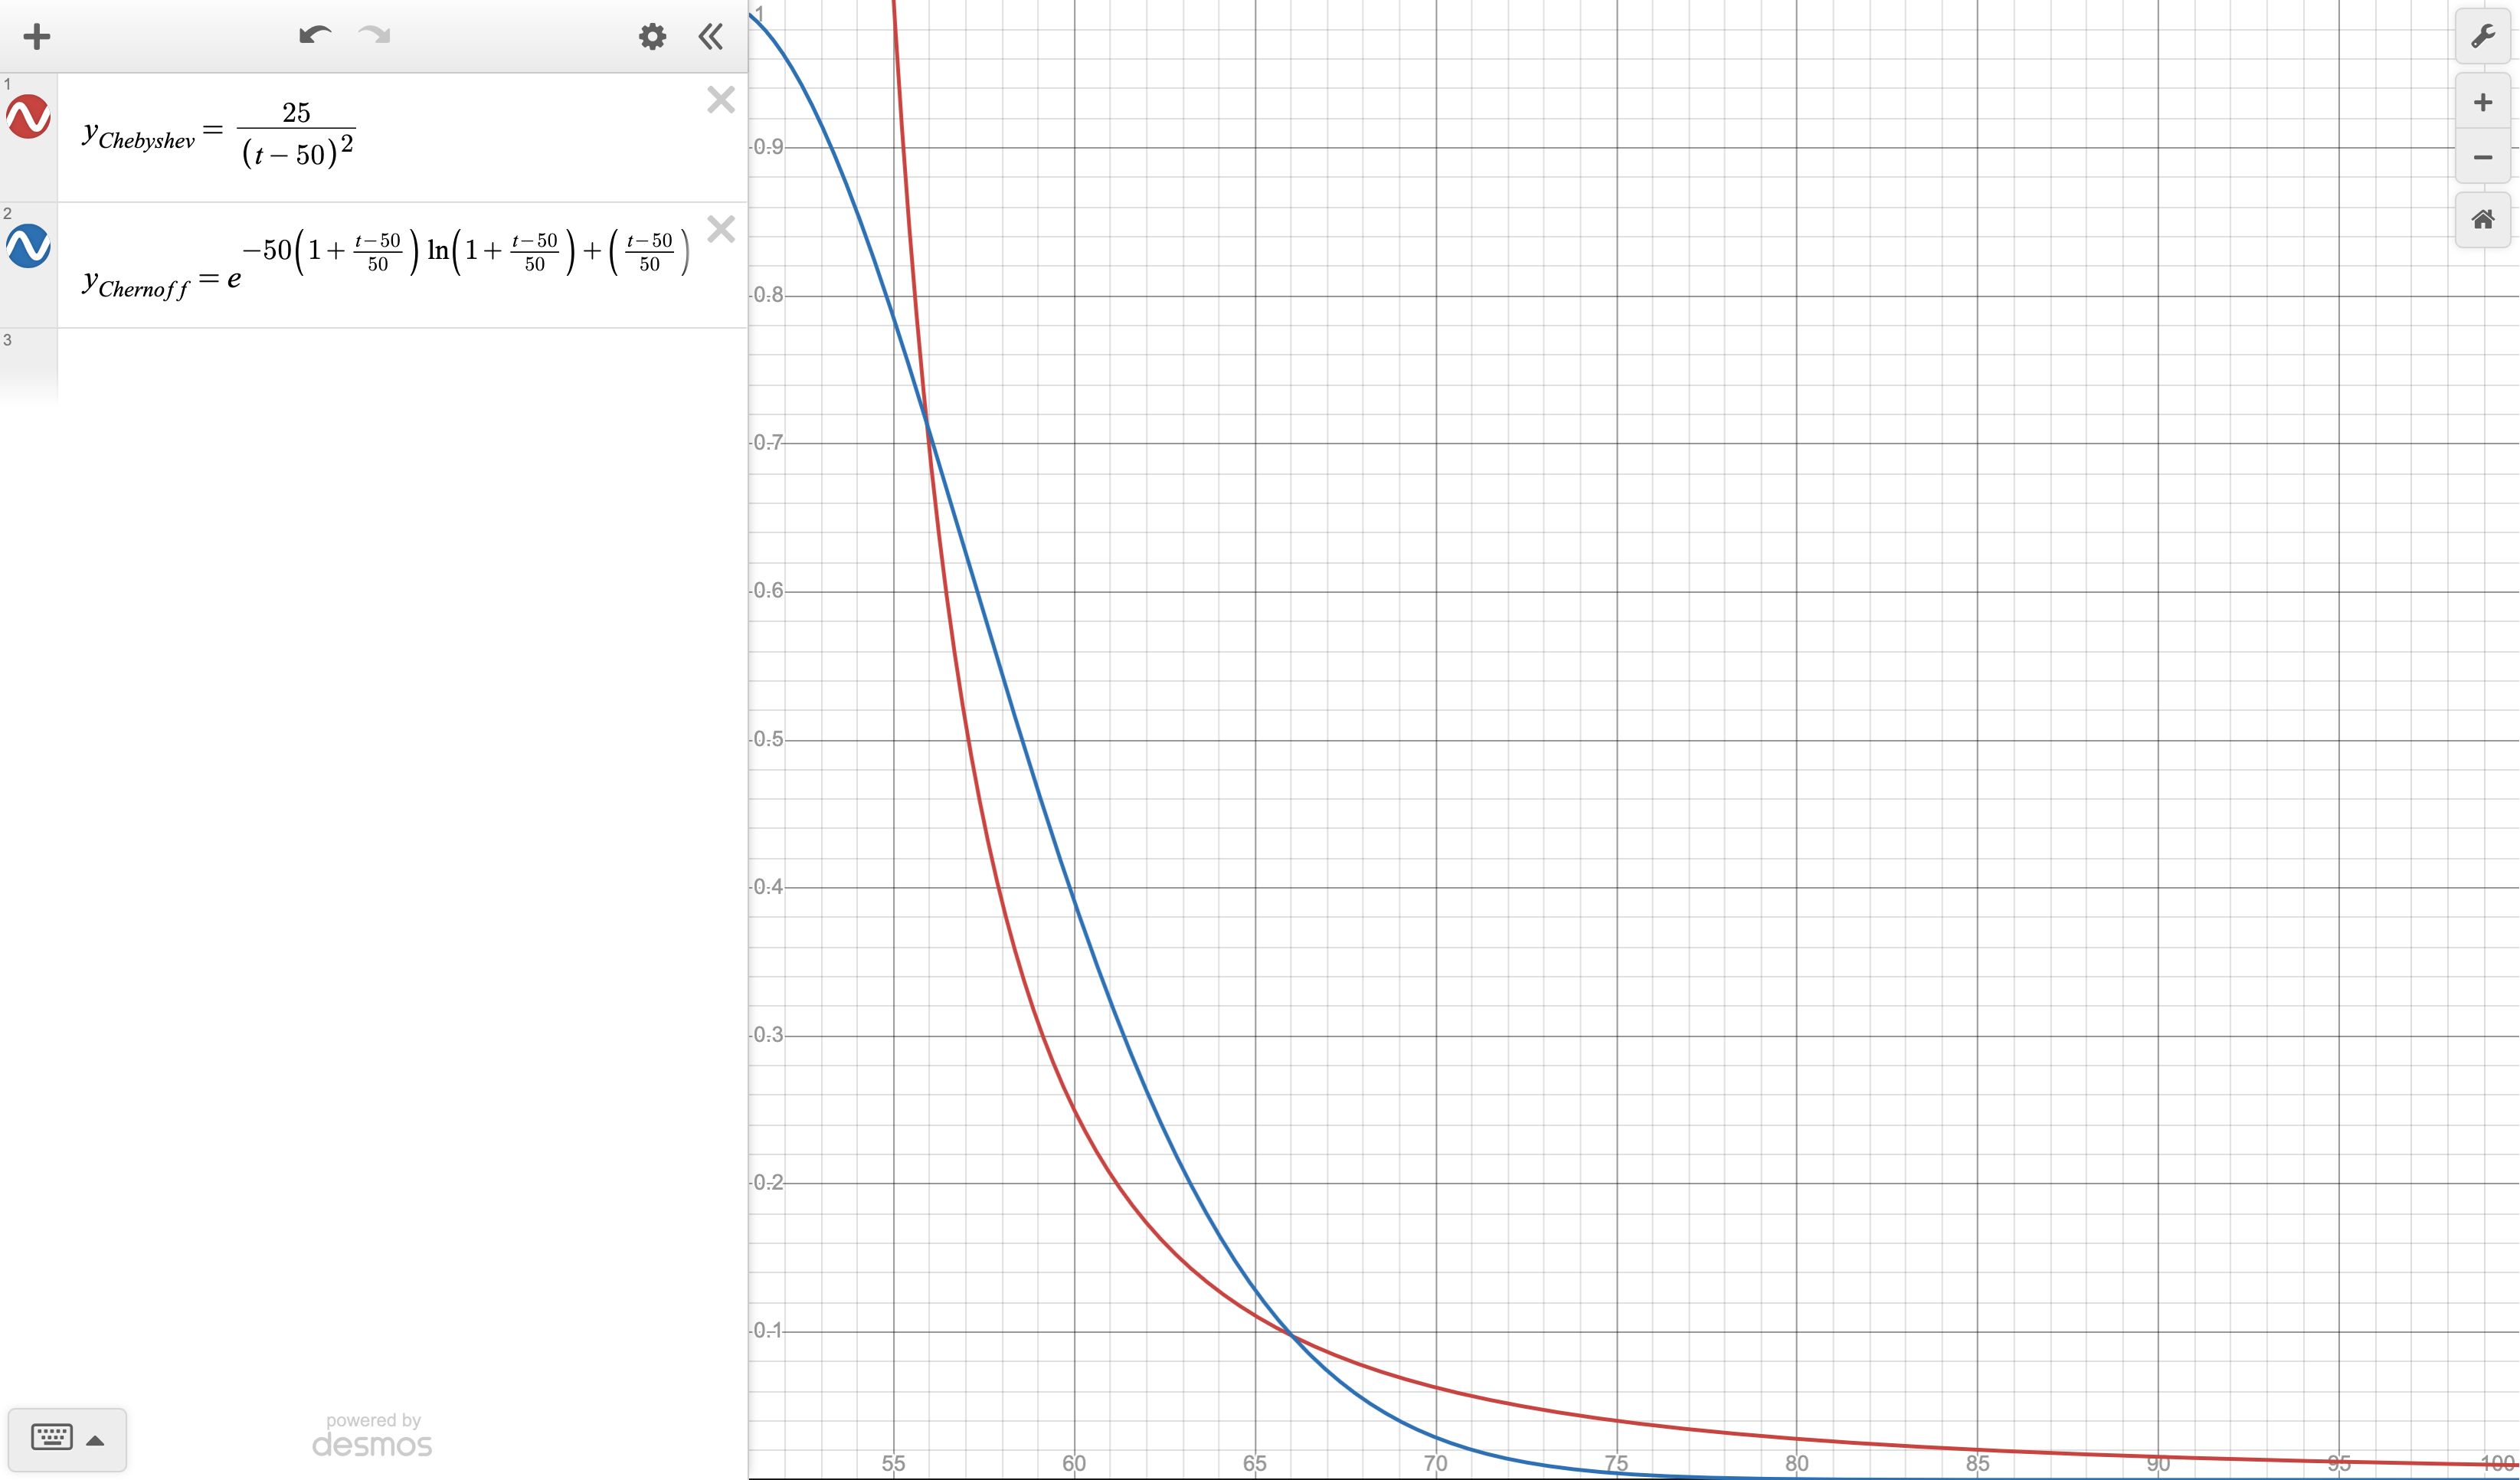
\includegraphics[width=0.95\textwidth]{graph.png} 
    \caption{Part (f) graph}
\end{figure}

Chebyshev is below Chernoff between roughly $56 \leq t \leq 66$, and above
elsewhere. The $\delta$ value is $\frac{t-50}{50}$. For Chebyshev, 
\[
    \Pr[X \geq t] = \Pr[X ]
\]

\end{Parts}

\end{solution}

\Question{Max of Uniforms}
\notelinks{\href{https://www.eecs70.org/assets/pdf/notes/n21.pdf}{Note 21}}
Let $X_1,...X_n$ be independent Uniform$(0,1)$ random variables, and let $X = 
\max(X_1,...X_n)$. Compute each of the following in terms of $n$.
\begin{Parts}
	\Part What is the cdf of $X$?
	\Part What is the pdf of $X$?
	\Part What is $\E[X]$?
	\Part What is $\Var(X)$?
\end{Parts}

\begin{solution}

\begin{Parts}
    
\Part The cumulative distribution function of $X$ is
\[
    \begin{split}
        F_X(t) &= \Pr[X < t] \\
        &= \Pr[X_1 < t] \cdot \Pr[X_2 < t] \cdots \Pr[X_n < t] \\
        &= F_{X_1}(t) \cdot F_{X_2}(t) \cdots F_{X_n}(t) \\
        &= \begin{cases}
            0, & \text{for } t < a \\
            \frac{(t-a)^n}{(b-a)^n}, & \text{for } a \leq t \leq b \\
            1, & \text{for } b < t
        \end{cases} \\
        &= \begin{cases}
            0, & \text{for } t < 0 \\
            t^n, & \text{for } 0 \leq t \leq 1 \\
            1, & \text{for } 1 < t
        \end{cases}
    \end{split}
\]

since all of $X_1, \dots X_n$ must be less than $t$ for $X$ to be less than $t$,
and the variables are independent and uniform over (0, 1).

\Part From the fundamental thereom of calculus,
\[
    \begin{split}
        \frac{d}{dt} F_X(t) &= \begin{cases}
            0, & \text{for } t < 0 \\
            n \cdot t^{n-1}, & \text{for } 0 \leq t \leq 1 \\
            0, & \text{for } 1 < t
        \end{cases} \\
        &= f_X(t)
    \end{split}
\]
and is the probability density function. 

\Part The expected value of $X$ is
\[
    \begin{split}
        \E[X] &= \int_{-\infty}^{\infty} t \cdot f_X(t) \, dt \\
        &= \int_{-\infty}^{0} 0 \, dt + \int_{0}^{1} n \cdot t^{n-1} \, dt + \int_{1}^{\infty} 0 \, dt \\
        &= \frac{n}{n+1} \left. (t^{n+1}) \right|_0^1 \\
        &= \frac{n}{n+1}.
    \end{split}
\]

\Part To find the variance of $X$, I will first find the expected value of 
$X^2$, which is
\[
    \begin{split}
        \E[X^2] &= \int_{-\infty}^{\infty} t^2 \cdot f_X(t) \, dt \\
        &= n \int_{0}^{1} t^2 \cdot t^{n-1}  \, dt \\
        &= \frac{n}{n+2} \left. (t^{n+1}) \right|_0^1 \\
        &= \frac{n}{n+2}.
    \end{split}
\]

Then, the variance of $X$ is
\[
    \Var(X) = \E[X^2] - (\E[X])^2 = \frac{n}{n+2} - \left( \frac{n}{n+1} \right)^2.
\]

\end{Parts}

\end{solution}

\Question{Short Answer}

\notelinks*{\href{https://www.eecs70.org/assets/pdf/notes/n21.pdf}{Note 21}}
\begin{Parts}
    \Part Let $X$ be uniform on the interval $[0,2]$, and define $Y = 4X^2 + 1$. 
    Find the PDF, CDF, expectation, and variance of $Y$.

    \Part Let $X$ and $Y$ have joint distribution 
    \[
        f(x,y) = \begin{cases}
            c x y + \frac{1}{4} & \text{$x \in [1,2]$ and $y \in [0,2]$} \\
            0 & \text{otherwise.}
        \end{cases}
    \]
    Find the constant $c$ (Hint: remember that the PDF must integrate to 1). Are 
    $X$ and $Y$ independent?

    \Part Let $X \sim \Exp(3)$. 
    \begin{Parts}
    	\item Find probability that $X \in [0, \,1]$.
    	\item Let $Y = \lfloor X \rfloor$, where the floor operator is defined 
        as:  $(\forall x \in [k, k+1))(\lfloor x \rfloor = k)$. For each $k \in 
        \N$, what is the probability that $Y = k$? Write the distribution of $Y$ 
        in terms of one of the famous distributions; provide that distribution's 
        name and parameters.
    \end{Parts}

    \Part Let $X_i \sim \Exp(\lambda_i)$ for $i = 1,\ldots,n$ be mutually 
    independent. It is a (very nice) fact that $\min(X_1,\ldots,X_n) \sim 
    \Exp(\mu)$. Find $\mu$.
\end{Parts}

\begin{solution}
    
\begin{Parts}
    
\Part The PDF and CDF of $X$ are
\[
    \begin{array}{c@{\hspace{3em}}c}
        \begin{split}
            f_X &= \begin{cases}
                0, & \text{for } t < 0 \\
                \frac{1}{2}, & \text{for } 0 \leq t \leq 2 \\
                0, & \text{for } 2 < t
            \end{cases}
        \end{split}
        &
        \begin{split}
            F_X &= \begin{cases}
                0, & \text{for } t < 0 \\
                \frac{t}{2}, & \text{for } 0 \leq t \leq 2 \\
                1, & \text{for } 2 < t               
            \end{cases}
        \end{split}
    \end{array}
\]

which can be used to find those for $Y$. The CDF of $Y$ in terms of $X$ is
\[
    \begin{split}
        F_Y(t) &= \Pr[Y < t] = \Pr[4X^2+1 < t] = \Pr[X < \sqrt{t-1}/2] \\
        &= \begin{cases}
            0, & \text{for } \sqrt{t-1}/2 < 0 \\
            \frac{\sqrt{t-1}}{4}, & \text{for } 0 \leq \sqrt{t-1}/2 \leq 2 \\
            1, & \text{for } 2 < \sqrt{t-1}/2
        \end{cases} \\
        &= \begin{cases}
            0, & \text{for } t < 1 \\
            \frac{\sqrt{t-1}}{4}, & \text{for } 1 \leq t \leq 17 \\
            1, & \text{for } 17 < t
        \end{cases}
    \end{split}
\]

from which the PDF can be found by taking the derivative:
\[
    \begin{split}
        \frac{d}{dt} F_Y(t) &= f_Y(t) \\
        &= \begin{cases}
            0, & \text{for } t < 1 \\
            \frac{1}{8\sqrt{t-1}}, & \text{for } 1 \leq t \leq 17 \\
            0, & \text{for } 17 < t.
        \end{cases}
    \end{split}
\]

The expected value and the variance of $Y$ are
\[
    \begin{array}{c@{\hspace{3em}}c}
        \begin{split}
            \E[Y] &= \E[4X^2+1] = 4\E[X^2] + 1 \\
            &= 4 \int_{0}^{2} t^2 \cdot \frac{1}{2} \, dt + 1 \\
            &= \frac{2}{3} \cdot 8 + 1 \\
            &= \frac{19}{3}
        \end{split}
        &
        \begin{split}
            \Var(Y) &= \E[Y^2] - \left( \E[Y] \right)^2 \\
            &= 16 \E[X^4] + 8 \E[X^2] + 1 - \left( \frac{19}{3} \right)^2 \\
            &= 16 \cdot \frac{32}{10} + 8 \cdot \frac{4}{3} + 1 - \left( \frac{19}{3} \right)^2 \\
            & \approx 22.756
        \end{split}
    \end{array}
\]

\Part The double integral of the joint distribution evaluates to 1, which
solves for the unknown $c$:
\[
    \begin{split}
        1 &= \int_{1}^{2} \int_{0}^{2} (cxy + \frac{1}{4}) \, dy dx \\
        &= \int_{1}^{2} (2cx + \frac{1}{2}) \, dx \\
        &= 4c + 1 - \left( c + \frac{1}{2} \right) \\
        1 &= 3c + \frac{1}{2} \\
        c &= \frac{1}{6}.
    \end{split}
\]

For independence, the product of the marginal PDFs for both $X$ and $Y$ must
equal the joint PDF above. The marginal PDFs are below: 
\[
    \begin{array}{c@{\hspace{3em}}c}
        \begin{split}
            f_X &= \int_{0}^{2} (\frac{1}{6}xy + \frac{1}{4}) \, dy \\
            &= \left. (\frac{1}{12}xy^2 + \frac{1}{4}y) \right|_0^2 \\
            &= \frac{1}{3}x + \frac{1}{2}
        \end{split}
        &
        \begin{split}
            f_Y &= \int_{1}^{2} (\frac{1}{6}xy + \frac{1}{4}) \, dx \\
            &= \left. (\frac{1}{12}x^2y+\frac{1}{4}x) \right|_1^2 \\
            &= \frac{1}{4}y + \frac{1}{4}.
        \end{split}
    \end{array}
\]

The product of the two is not equal to the original:
\[
    f_X \cdot f_Y = \left( \frac{1}{3}x + \frac{1}{2} \right) 
    \left( \frac{1}{4}y + \frac{1}{4} \right) \neq \frac{1}{6}xy+\frac{1}{4} = f_{X,Y}
\]

so they are not independent. 

\Part The probability that $X \in [0, 1]$ is
\[
    \begin{split}
        \Pr[0 \leq X \leq 1] &= \int_{0}^{1} 3e^{-3t} \, dt \\
        &= 3 \cdot -\frac{1}{3} \left. (e^{-3t}) \right|_0^1 \\
        &= 1-e^{-3}. \\
    \end{split}
\]

The probability that $Y=k$ is the exact same as the probability that 
$X \in [k, k+1)$ or $k \leq X < k+1$. So, 
\[
    \begin{split}
        \Pr[Y=k] &= \Pr[k \leq X < k+1] \\
        &= \Pr[X < k+1] - \Pr[X < k] \\
        &= F_X(k+1) - F_X(k) \\
        &= (1-e^{-3(k+1)}) - (1-e^{-3k}) \\
        &= e^{-3k + 3} + e^{-3k} \\
        &= e^{-3k}(-e^3+1) \\
    \end{split}
\]
and $Y$ is a random variable following a geometric distribution with probability
of success $p=1-e^3$. 

\Part We can find the parameter by finding the CDF of $\min(X_1, \dots, X_n)$:
\[
    ]\begin{split}
        \Pr[\min(X_1, \dots, X_n)] &= 1 - \Pr[X_1 > k, \dots, X_n > k] \\
        &= 1 - \Pr[X_1 > k] \cdots \Pr[X_n > k] \\
        &= 1 - e^{-\lambda_1 k} \cdots e^{-\lambda_n k} \\
        &= 1 - e^{-(\lambda_1 + \dots + \lambda_n) k} \\
    \end{split}
\]

which takes on the same form as $F_X(t) = 1 - e^{-\lambda t}$, and so $\mu = 
\lambda_1 + \dots + \lambda_n$.

\end{Parts}

\end{solution}

\Question{Darts with Friends}

\notelinks{\href{https://www.eecs70.org/assets/pdf/notes/n21.pdf}{Note 21}}
Michelle and Alex are playing darts.
Being the better player, Michelle's aim follows a uniform distribution over a 
disk of radius $1$ around the center. Alex's aim follows a uniform distribution 
over a disk of radius $2$ around the center. 

\begin{Parts}
    \Part Let the distance of Michelle's throw from the center be denoted by the 
    random variable $X$ and let the distance of Alex's throw from the center be 
    denoted by the random variable $Y$.
    \begin{enumerate}
    \item[(i)] What's the cumulative distribution function of $X$?
    \item[(ii)] What's the cumulative distribution function of $Y$?
    \item[(iii)] What's the probability density function of $X$?
    \item[(iv)] What's the probability density function of $Y$?
    \end{enumerate}
    
    \Part What's the probability that Michelle's throw is closer to the center 
    than Alex's throw? What's the probability that Alex's throw is closer to 
    the center? 
    
    \Part What's the cumulative distribution function of $U = \max(X,Y)$?
        
\end{Parts}

\begin{solution}
    
\begin{Parts}
    
\Part The CDF of $X$ is $F_X(r) = \Pr[X < r] = \frac{\pi r^2}{\pi \cdot 1^2} = 
r^2$. The CDF of $Y$ is $F_Y(r) = \Pr[Y < r] = \frac{\pi r^2}{\pi \cdot 4} = 
\frac{r^2}{4}$. The PDF of $X$ is then $2r$, and the PDF of $Y$ is then 
$\frac{r}{2}$.

\Part The probability that Michelle throws closer to Alex is 
\[
    \begin{split}
        \Pr[X < Y] &= \int_{0}^{2} \Pr[X < Y \mid Y = y] \Pr[Y = y] \, dy \\
        &= \int_{0}^{1} y^2 \cdot \frac{y}{2} \, dy + \int_{1}^{2} 1 \cdot \frac{y}{2} \, dy \\
        &= \frac{1}{2} \cdot \frac{1}{4} + \frac{1}{2} \cdot \left( 2- \frac{1}{2} \right) \\
        &= \frac{7}{8}
    \end{split}
\]

since it is guaranteed Michelle's throw will be closer than Alex's after $r=1$,
and before it is the CDF given Alex's throw. The probability that Alex's throw 
is closer to the center is the complement of this probability so $\Pr[Y < X] = 
\frac{1}{8}$.

\Part The CDF of $U$ is $\Pr[U < r] = \Pr[X < r, Y < r]$ since both need to be 
less than to evade the maximum selector function. So, $\Pr[X < r, Y < r] = 
\Pr[X < r] \cdot \Pr[Y < r]$ given independence. Although this varies depending
on what $r$ is in question, i.e., 
\[
    F_U(r) = \begin{cases}
        r^2 \times \frac{r^2}{4}, & \text{for } r < 1 \\
        \frac{r^2}{4}, & \text{for } 1 \leq r \leq 2 \\
        1, & \text{for } 2 < r
    \end{cases}
\]

\end{Parts}

\end{solution}

\end{document}
